\chapter{Les tests agiles}
\thispagestyle{fancy}
\section{ le testing agile et ses objectifs}
\label{sec:agiletest}
En général, les équipes de test cherchent à découvrir autant de bogues que possible dans le code développé, car les développeurs n'accordent que peu d'attention à la qualité. Les conséquences sont plus difficiles et coûteuses à corriger. Les équipes de test utilisent des outils pour documenter les cas de test et les bogues et peuvent externaliser la main-d'œuvre, mais cela ne résout pas les problèmes systémiques. Les activités de test intensives ralentissent la livraison et compromettent la qualité, souvent en raison de la pression de livraison tardive des projets et du manque de temps de test. Les défauts découverts à la dernière minute entraînent des retouches coûteuses et des problèmes plus graves si c'est un problème d'architecture ou de conception. Les équipes accumulent également une dette technique qui peut causer des retards futurs. La solution serait de déplacer les tests à des phases plus précoces du cycle de développement.
\begin{center}
    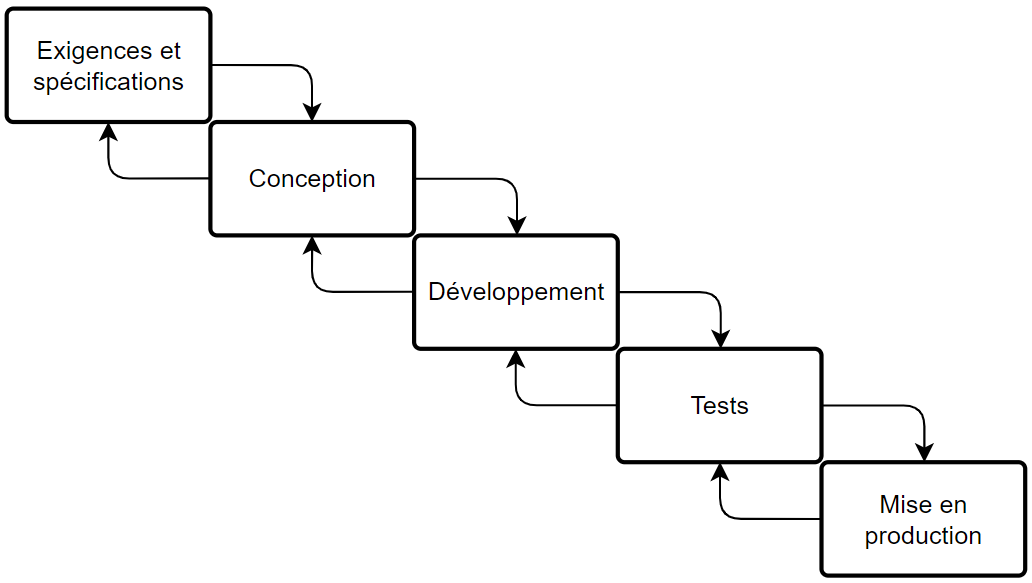
\includegraphics[width=0.7\textwidth]{incremental.png}

\end{center}
\section{valeurs fondamentales de l'agilité s'appliquent à l'approche de testing agile.}
\label{sec:testagile}
